\documentclass[11pt]{article}
\usepackage[a4paper,margin=2.3cm]{geometry}
\usepackage[T1]{fontenc}
\usepackage[utf8]{inputenc}
\usepackage{lmodern}
\usepackage{microtype}
\usepackage{graphicx}
\usepackage{booktabs}
\usepackage{tabularx}
\usepackage{array}
\usepackage{ragged2e}
\usepackage{xcolor}
\usepackage{enumitem}
\usepackage[font=small,labelfont=bf]{caption}
\usepackage{titlesec}
\usepackage{fancyhdr}
\usepackage{lastpage}
\usepackage{xurl}
\usepackage[colorlinks=true,linkcolor=deep,urlcolor=accent,citecolor=deep]{hyperref}

% Generated by docs/build_figures.py. Do not edit by hand.
\newcommand{\nBuildDate}{19 October 2026}
\newcommand{\nEvDate}{31 August 2026}
\newcommand{\nPopYear}{2023}
\newcommand{\nNDeps}{100}
\newcommand{\nRawRows}{157,460}
\newcommand{\nRawCols}{52}
\newcommand{\nDupRemoved}{7,919}
\newcommand{\nDupGroups}{7,276}
\newcommand{\nDupCrossShare}{100}
\newcommand{\nAfterDup}{149,541}
\newcommand{\nPlaceholderRows}{119}
\newcommand{\nNoDepRemoved}{213}
\newcommand{\nCleanRows}{149,328}
\newcommand{\nWattsConverted}{4}
\newcommand{\nZeroPower}{2,709}
\newcommand{\nSuspiciousPower}{289}
\newcommand{\nSuspiciousKw}{400}
\newcommand{\nDateBeforeMin}{33}
\newcommand{\nDateFuture}{1}
\newcommand{\nDateMissing}{65,211}
\newcommand{\nDateMissingPct}{44}
\newcommand{\nDatedPct}{56}
\newcommand{\nInseeMissingPct}{41}
\newcommand{\nDepByInsee}{87,439}
\newcommand{\nDepByCoords}{61,889}
\newcommand{\nDepCheckRows}{87,197}
\newcommand{\nDepAgreePct}{99.0}
\newcommand{\nCoordsOutside}{170}
\newcommand{\nOperatorsDistinct}{292}
\newcommand{\nTopN}{12}
\newcommand{\nEvRows}{773,782}
\newcommand{\nEvNoDep}{0}
\newcommand{\nEvQuarters}{22}
\newcommand{\nFrPoints}{149,328}
\newcommand{\nFrPerHundredK}{219}
\newcommand{\nFrPerHundredEv}{5.4}
\newcommand{\nFrKwPerEv}{3.0}
\newcommand{\nFrFastShare}{37}
\newcommand{\nFrFastPerHundredK}{81}
\newcommand{\nMainPerHundredK}{225}
\newcommand{\nOverPerHundredK}{34}
\newcommand{\nOverPoints}{663}
\newcommand{\nOverPop}{1,928,465}
\newcommand{\nLowestName}{Guyane}
\newcommand{\nLowestPoints}{1}
\newcommand{\nLowestPop}{293,996}
\newcommand{\nHighestName}{Hautes-Alpes}
\newcommand{\nHighestPerHundredK}{452}
\newcommand{\nNBelowFr}{52}
\newcommand{\nTopTenPointsShare}{29}
\newcommand{\nTopTenPopShare}{25}
\newcommand{\nEvFirst}{414,942}
\newcommand{\nEvLast}{2,756,113}
\newcommand{\nEvFirstDate}{December 2020}
\newcommand{\nEvLastDate}{August 2026}
\newcommand{\nEvFold}{6.6}
\newcommand{\nNTwentyTwenty}{1,895}
\newcommand{\nNTwentyTwentyOne}{8,897}
\newcommand{\nPeakN}{18,256}
\newcommand{\nPeakYear}{2023}
\newcommand{\nLastFullN}{11,830}
\newcommand{\nLastFullYear}{2025}
\newcommand{\nStartYear}{2023}
\newcommand{\nPivotYear}{2022}
\newcommand{\nEndYear}{2026}
\newcommand{\nEndMonth}{October 2026}
\newcommand{\nAddedPeriod}{56,657}
\newcommand{\nGrowthPeriod}{205}
\newcommand{\nRuralPerHundredK}{226}
\newcommand{\nDensePerHundredK}{222}
\newcommand{\nRuralFastPerHundredK}{87}
\newcommand{\nDenseFastPerHundredK}{76}
\newcommand{\nRuralPerHundredEv}{7.2}
\newcommand{\nDensePerHundredEv}{4.9}
\newcommand{\nRuralN}{31}
\newcommand{\nDenseN}{28}
\newcommand{\nRuralUltra}{36}
\newcommand{\nDenseUltra}{27}
\newcommand{\nRuralMax}{60}
\newcommand{\nDenseMin}{150}
\newcommand{\nConvBefore}{5.8}
\newcommand{\nConvAfter}{2.2}
\newcommand{\nConvLowBefore}{13}
\newcommand{\nConvLowAfter}{74}
\newcommand{\nConvHighBefore}{77}
\newcommand{\nConvHighAfter}{167}
\newcommand{\nOverAdded}{10}
\newcommand{\nOverPace}{0.1}
\newcommand{\nMainPace}{22.5}
\newcommand{\nSlowestName}{Seine-Saint-Denis}
\newcommand{\nSlowestYears}{11}
\newcommand{\nSlowestPace}{10.1}
\newcommand{\nNBelowAfir}{5}
\newcommand{\nBelowAfirNames}{Guyane, Martinique, La Réunion, Guadeloupe, Hauts-de-Seine}
\newcommand{\nAfirLow}{0.8}
\newcommand{\nAfirHigh}{1.3}
\newcommand{\nRhoEv}{$-$0.37}
\newcommand{\nDenseLowName}{Seine-Saint-Denis}
\newcommand{\nDenseLowPerHundredK}{106}
\newcommand{\nDenseLowEvNames}{Hauts-de-Seine, Yvelines, Seine-Saint-Denis}
\newcommand{\nDenseLowEvValues}{2.5, 2.7, 3.2}
\newcommand{\nDenseLowEvFirst}{Hauts-de-Seine}
\newcommand{\nDenseLowEvFirstValue}{2.5}
\newcommand{\nParisPerHundredK}{320}
\newcommand{\nParisFastShare}{5}
\newcommand{\nUltraDedicatedShare}{44}
\newcommand{\nMapSample}{12,000}
\newcommand{\nSeed}{42}
\newcommand{\nUltraShareTwentyOne}{6}
\newcommand{\nUltraShareLastFull}{33}


\definecolor{deep}{HTML}{000000}
\definecolor{accent}{HTML}{000000}
\definecolor{muted}{HTML}{000000}

\titleformat{\section}{\large\bfseries\color{deep}}{\thesection}{0.6em}{}
\titleformat{\subsection}{\normalsize\bfseries\color{deep}}{\thesubsection}{0.6em}{}
\setlist{itemsep=2pt,topsep=4pt}
\newcolumntype{Y}{>{\RaggedRight\arraybackslash}X}
\setlength{\parskip}{4pt}

\pagestyle{fancy}
\fancyhf{}
\renewcommand{\headrulewidth}{0pt}
\fancyfoot[L]{\footnotesize\color{muted}Public EV charging in France. Oscar Masdupuy}
\fancyfoot[R]{\footnotesize\color{muted}\thepage/\pageref{LastPage}}

\newcommand{\headline}[1]{\par\noindent{\color{deep}\bfseries #1}\par}

\begin{document}

\begin{center}
{\LARGE\bfseries\color{deep} Public EV charging in France:\\[2pt] where it lags, and how fast the gap is closing}\\[8pt]
{\large Oscar Masdupuy}\\[2pt]
{\color{muted}EFREI Paris, 4th year, Business Intelligence \& Analytics (BIA). Data Visualization 2026}\\[2pt]
{\color{muted}Code: \url{https://github.com/Masdupp/Public-EV-charging-in-France}. Data of \nBuildDate.}\\[2pt]
{\small\itshape Formatting with the help of AI.}
\end{center}

\vspace{4pt}
\noindent\fcolorbox{accent}{white}{\parbox{\dimexpr\linewidth-2\fboxsep-2\fboxrule}{\small
\textbf{Summary.} This report documents a Streamlit app built on the national file of public charging points (IRVE) published on data.gouv.fr. It addresses département and regional planners and tests a common assumption: that charging sped up after 2021 but stayed in big cities, leaving rural départements short of fast chargers. The data supports the first half and contradicts the second. Rural mainland départements have \nRuralPerHundredK{} points per 100,000 inhabitants against \nDensePerHundredK{} in dense ones, and the ratio between the best and least equipped quarter of départements fell from \nConvBefore{} to \nConvAfter{} between \nPivotYear{} and \nEndYear. The gaps that remain are overseas (\nOverPerHundredK{} points per 100,000 people against \nMainPerHundredK{} on the mainland) and, per rechargeable car, in dense départements around Paris.}}

\section{Problem and audience}

The stock of rechargeable cars in France went from \nEvFirst{} in \nEvFirstDate{} to \nEvLast{} in \nEvLastDate, a \nEvFold-fold increase. Drivers without a private parking space, and anyone on a long trip, depend on public charging.

Since the 2019 mobility law (LOM), départements, intercommunalities and energy syndicates can write a master plan for public charging (schéma directeur IRVE, or SDIRVE). The people who write these plans need a fair comparison of their territory with the rest of the country. Raw counts are not fair: Paris has many points because it has many people. The app therefore compares départements per inhabitant and per rechargeable car.

It answers two questions:
\begin{enumerate}
  \item Where is public charging thin once population and EV ownership are taken into account?
  \item Is the gap between the best and least equipped départements closing, and how fast?
\end{enumerate}

The working hypothesis was that deployment accelerated after 2021 but stayed concentrated in large metropolitan areas and along motorways, leaving rural départements behind on fast charging.

\section{Data}

All sources are listed on data.gouv.fr. The download script asks the data.gouv.fr API for each dataset's current resources instead of using a fixed file URL, because the IRVE file is regenerated every day under a new name.

\begin{table}[h]
\centering\small
\begin{tabularx}{\linewidth}{@{}p{4.6cm}Yp{2.6cm}@{}}
\toprule
\textbf{Dataset} & \textbf{Content and use} & \textbf{Licence} \\
\midrule
Base nationale des IRVE, consolidated static file & One row per charging point (\nRawRows{} rows, \nRawCols{} columns): operator, power, coordinates, commune code, commissioning date. Schema \texttt{etalab/schema-irve-statique}. & Licence Ouverte 2.0 \\
Voitures particulières immatriculées par commune et par type de recharge & Agence ORE, from the SDES vehicle register. Rechargeable cars per commune, \nEvQuarters{} snapshots since December 2020. & Licence Ouverte 2.0 \\
Populations de référence & Insee, municipal population \nPopYear{} per département. & Licence Ouverte 2.0 \\
Contours administratifs & Département shapes (2025), used for the map and to place points from their coordinates. & ODbL 1.0 \\
\bottomrule
\end{tabularx}
\caption{Sources. Full URLs and download dates are in \texttt{data/SOURCES.md}.}
\end{table}

The vehicle file joined on the INSEE commune code with \nEvNoDep{} unmatched rows out of \nEvRows. Mayotte is the only département left out, because the Insee \nPopYear{} reference file has no population for it. The analysis covers \nNDeps{} départements.

\section{Cleaning and validation}

\begin{table}[h]
\centering\small
\begin{tabularx}{\linewidth}{@{}Yrr@{}}
\toprule
\textbf{Step} & \textbf{Rows removed} & \textbf{Rows left} \\
\midrule
Raw file & & \nRawRows \\
Duplicate \texttt{id\_pdc\_itinerance}, kept the row with the latest update date & \nDupRemoved & \nAfterDup \\
No usable commune code and coordinates outside every département & \nNoDepRemoved & \nCleanRows \\
\bottomrule
\end{tabularx}
\caption{From raw file to analysis table.}
\end{table}

\textbf{Duplicates.} \nDupGroups{} charging-point IDs appeared more than once. In \nDupCrossShare\% of cases the copies came from different source files, typically a roaming aggregator and the operator publishing the same point. Keeping the most recent update assumes the newest declaration describes the point as it is today. \nPlaceholderRows{} rows use the placeholder ID ``Non concerné'' allowed by the schema; they were checked for duplicates on their content instead of their ID.

\textbf{Power.} The schema expects kW. \nWattsConverted{} values of 1,000 or more were read as watts and divided by 1,000. \nZeroPower{} points declared 0 kW and are reported as ``unknown power''. \nSuspiciousPower{} points above \nSuspiciousKw{} kW were kept, since they fall in the ultra-fast class either way, and flagged in the app. Power classes follow the brief: slow below 7.4 kW, normal from 7.4 to 22 kW, fast above 22 and below 150 kW, ultra-fast from 150 kW. A 22 kW wallbox counts as normal, because 22 kW is the standard AC rating.

\textbf{Commissioning date.} \nDateBeforeMin{} dates before 2010 (1900, 1947, 2002) and \nDateFuture{} date in the future were set to missing. In total \nDateMissing{} points (\nDateMissingPct\%) have no usable date.

\textbf{Département.} The commune code is empty in \nInseeMissingPct\% of raw rows. The département comes from the commune code when it is valid (\nDepByInsee{} points), and otherwise from a point-in-polygon test of the coordinates against the département shapes (\nDepByCoords{} points). On the \nDepCheckRows{} points where both methods work, they agree \nDepAgreePct\% of the time, which validates the fallback.

\textbf{Operators and siting.} Operator names were upper-cased, roaming suffixes removed and obvious variants merged, leaving \nOperatorsDistinct{} operators; the app keeps the top \nTopN{} and groups the rest. The siting field had five spellings of the same category because of encoding errors; they were merged and translated.

\section{Indicators and method}

\begin{itemize}
  \item \textbf{Points per 100,000 inhabitants} and \textbf{fast points per 100,000}: the main fairness measure.
  \item \textbf{Points per 100 rechargeable cars} and \textbf{kW of public power per car}: demand-side measures. AFIR, the EU regulation on charging infrastructure, sets fleet targets of \nAfirHigh{} kW per battery car and \nAfirLow{} kW per plug-in hybrid. The register mixes both, so the app shows the range as a reference band, not a compliance test.
  \item \textbf{Density bands}: population over area at département level. Rural below \nRuralMax{} inhabitants per km², dense above \nDenseMin, intermediate between. The edges sit near the terciles.
  \item \textbf{Convergence}: départements are split into four groups by dated points per 100,000 inhabitants at the end of \nPivotYear. Each group's level then is compared with its level today, on the same dated subset.
  \item \textbf{Years to reach the France level}: gap to today's national rate divided by the département's pace over the period. It is a projection under stated assumptions, not a forecast.
\end{itemize}

Ratios over a group of départements are always ratios of sums (total points over total population), never averages of ratios. All aggregates are computed in the app from a table of \nCleanRows{} points, so every number on screen follows the filters.

\section{Findings}

\subsection{Deployment accelerated after 2021}
\headline{Dated commissioning went from \nNTwentyTwenty{} points in 2020 to \nNTwentyTwentyOne{} in 2021 and peaked at \nPeakN{} in \nPeakYear.}

\begin{figure}[h]
\centering
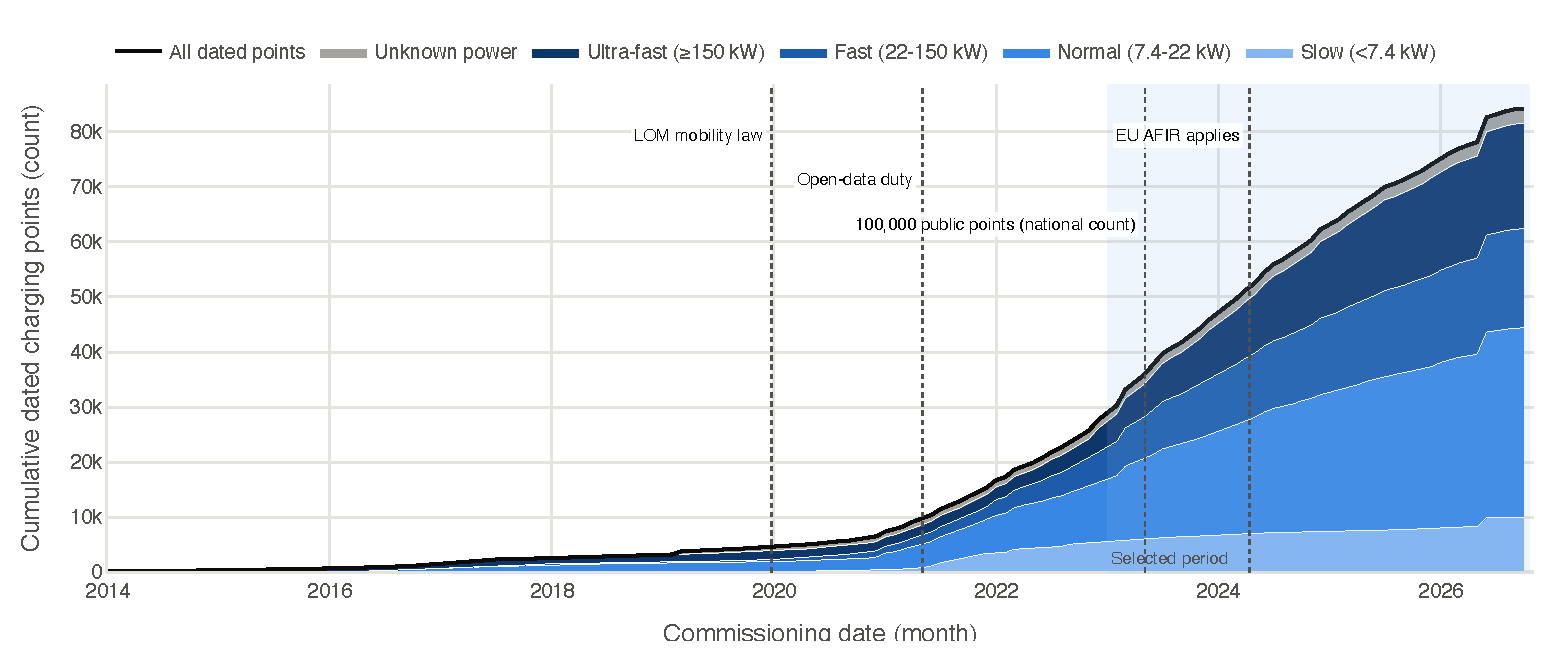
\includegraphics[width=\linewidth]{figures/timeline.pdf}
\caption{Cumulative dated charging points by power class. Dotted lines mark the LOM law (December 2019), the duty to publish IRVE data (May 2021), the national 100,000-point milestone (May 2023) and the start of AFIR (April 2024).}
\end{figure}

The first half of the hypothesis holds. \nLastFullYear{} added \nLastFullN{} dated points, fewer than the peak, but late publication may explain part of that drop. The 2021 jump coincides with the arrêté of 4 May 2021 that made publication mandatory, so some of it may reflect better reporting rather than more chargers. Ultra-fast points made up \nUltraShareTwentyOne\% of dated points commissioned in 2021 and \nUltraShareLastFull\% in \nLastFullYear{} (the darkest band).

\subsection{Where the gaps are}
\headline{\nHighestName{} leads with \nHighestPerHundredK{} points per 100,000 inhabitants; \nLowestName{} lists \nLowestPoints{} point for \nLowestPop{} people.}

\begin{figure}[h]
\centering
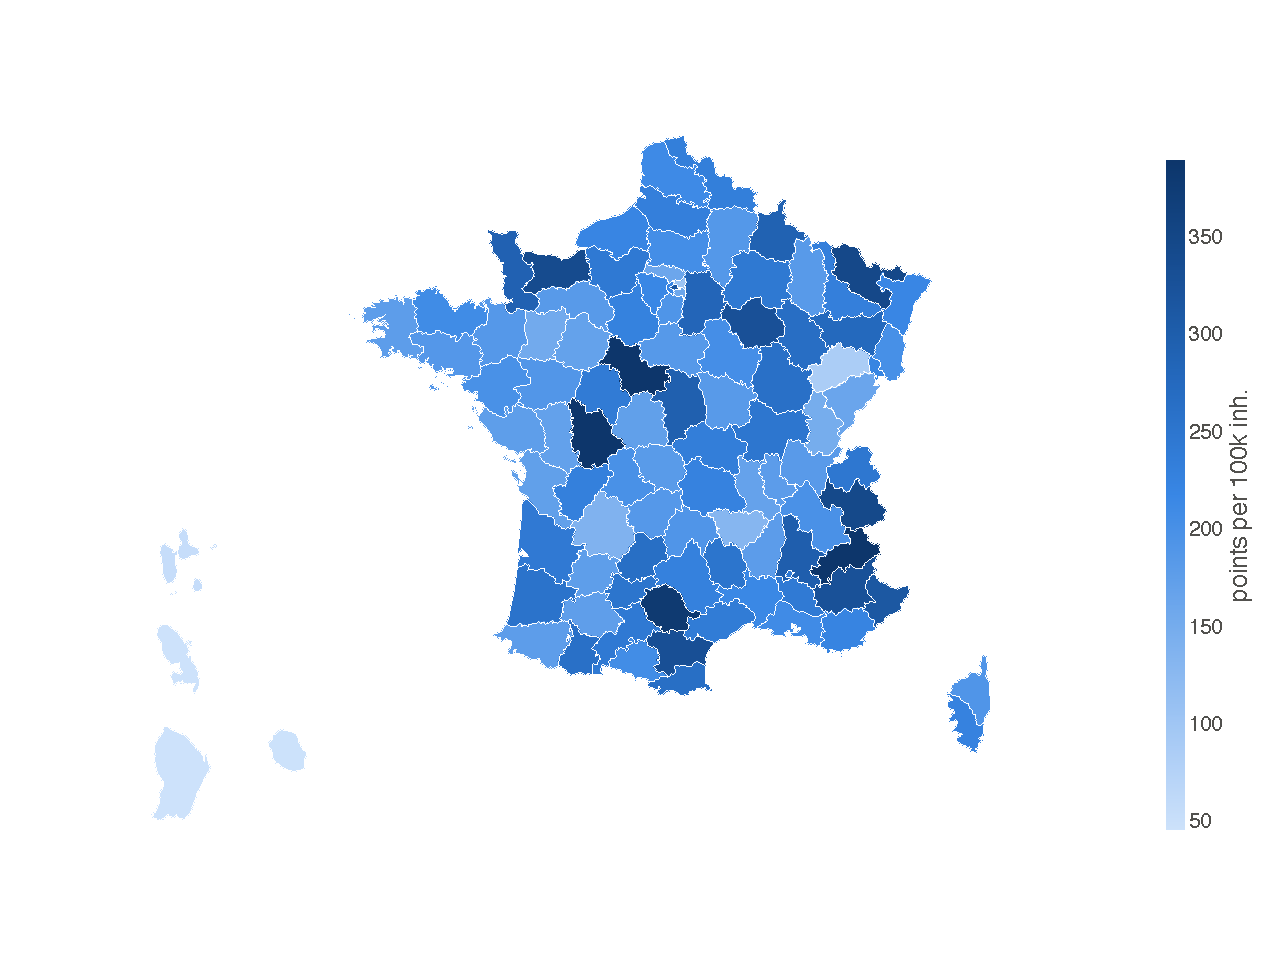
\includegraphics[width=0.66\linewidth,trim=60 60 0 55,clip]{figures/map.pdf}
\caption{Charging points per 100,000 inhabitants. Overseas départements are drawn as insets to the west.}
\end{figure}

\nNBelowFr{} of the \nNDeps{} départements sit below the national figure of \nFrPerHundredK. Deployment is only mildly concentrated: the 10 départements with the most points hold \nTopTenPointsShare\% of them for \nTopTenPopShare\% of the population. The four overseas départements stand apart, with \nOverPoints{} points for \nOverPop{} inhabitants.

\subsection{Rural départements are not behind}
\headline{Rural mainland départements have \nRuralPerHundredK{} points per 100,000 inhabitants against \nDensePerHundredK{} in dense ones, and \nRuralFastPerHundredK{} fast points against \nDenseFastPerHundredK.}

\begin{figure}[h]
\centering
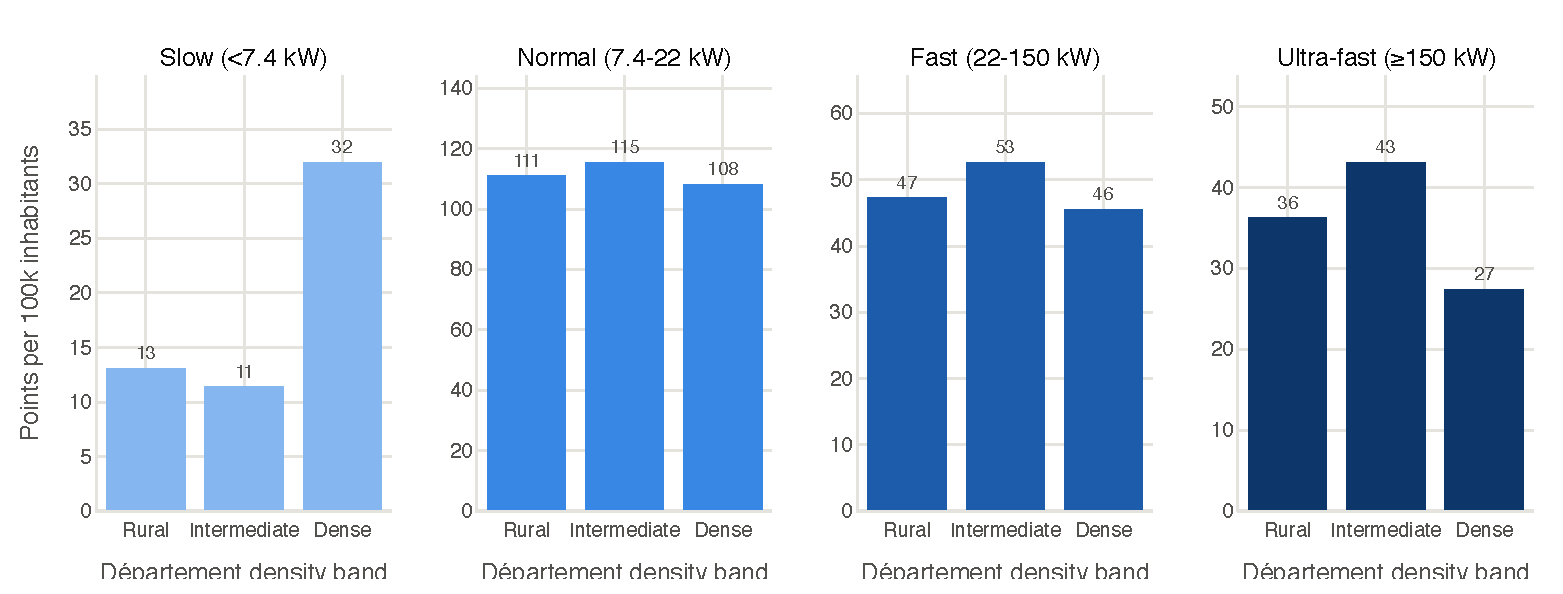
\includegraphics[width=\linewidth]{figures/density.pdf}
\caption{Points per 100,000 inhabitants by density band, one panel per power class (all \nNDeps{} départements). Each panel has its own scale.}
\end{figure}

The second half of the hypothesis does not hold. Dense départements lead only on slow charging. On ultra-fast charging, rural départements have \nRuralUltra{} points per 100,000 people against \nDenseUltra. Per rechargeable car the rural advantage is larger: \nRuralPerHundredEv{} points per 100 cars against \nDensePerHundredEv. Whether these fast chargers follow motorway corridors cannot be tested, because the file has no road layer.

\subsection{Charging measured against EV ownership}
\headline{Only \nNBelowAfir{} départements offer less than \nAfirLow{} kW of public power per rechargeable car: \nBelowAfirNames.}

\begin{figure}[h]
\centering
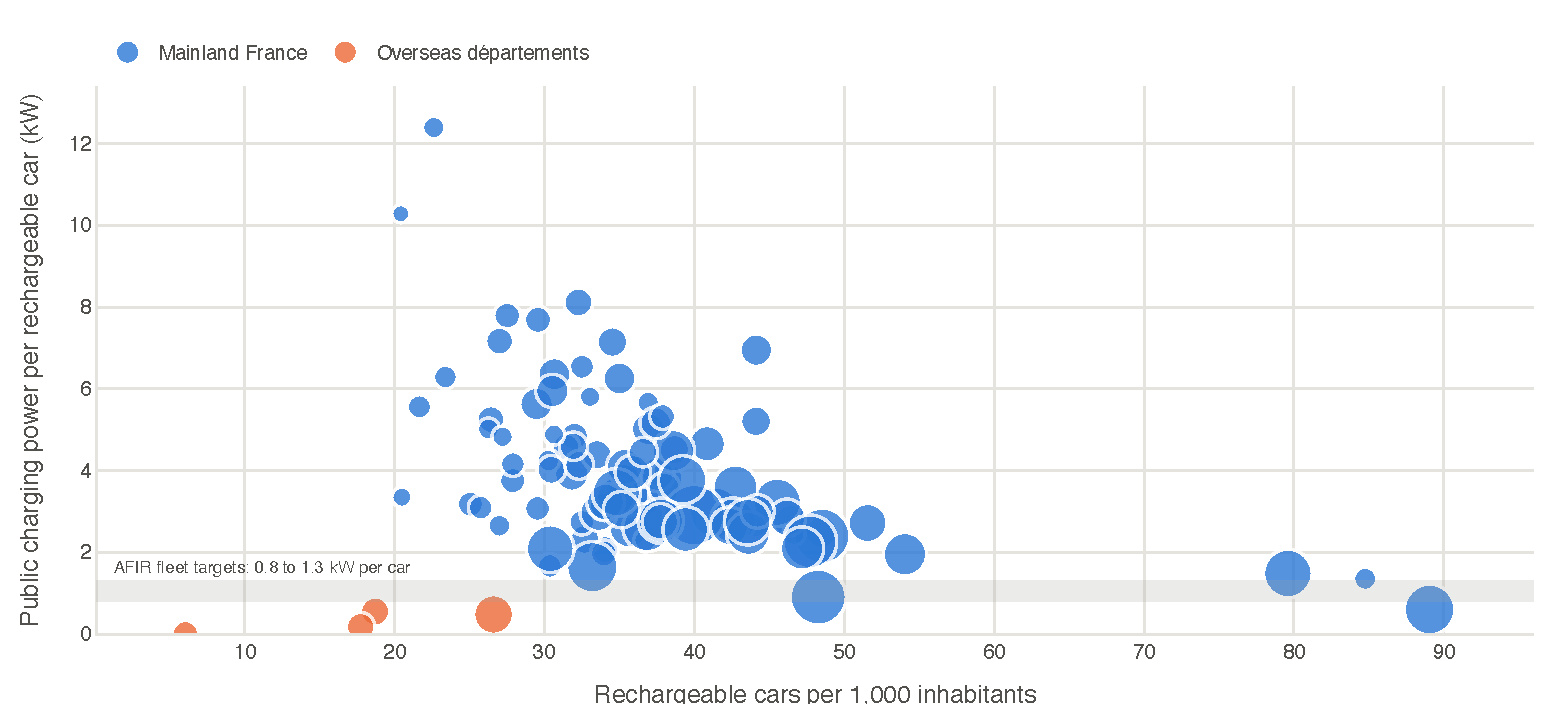
\includegraphics[width=0.92\linewidth]{figures/scatter.pdf}
\caption{Public charging power per rechargeable car against cars per 1,000 inhabitants. Bubble size follows population. Grey band: AFIR references.}
\end{figure}

France as a whole offers \nFrKwPerEv{} kW per rechargeable car. Départements with more EVs per inhabitant have fewer public points per car (Spearman rank correlation \nRhoEv). This is a correlation: home and workplace charging, which the file does not cover, are likely more common where ownership is high. The lowest per-car figures among dense départements are in \nDenseLowEvNames{} (\nDenseLowEvValues{} points per 100 cars, France \nFrPerHundredEv). Company and leasing cars registered at head offices inflate their car counts, so part of this gap is a measurement effect.

\subsection{The gap is closing on the mainland, not overseas}
\headline{The best equipped quarter of départements had \nConvBefore{} times more dated points per inhabitant than the least equipped quarter at the end of \nPivotYear; in \nEndMonth{} the ratio was \nConvAfter.}

\begin{figure}[h]
\centering
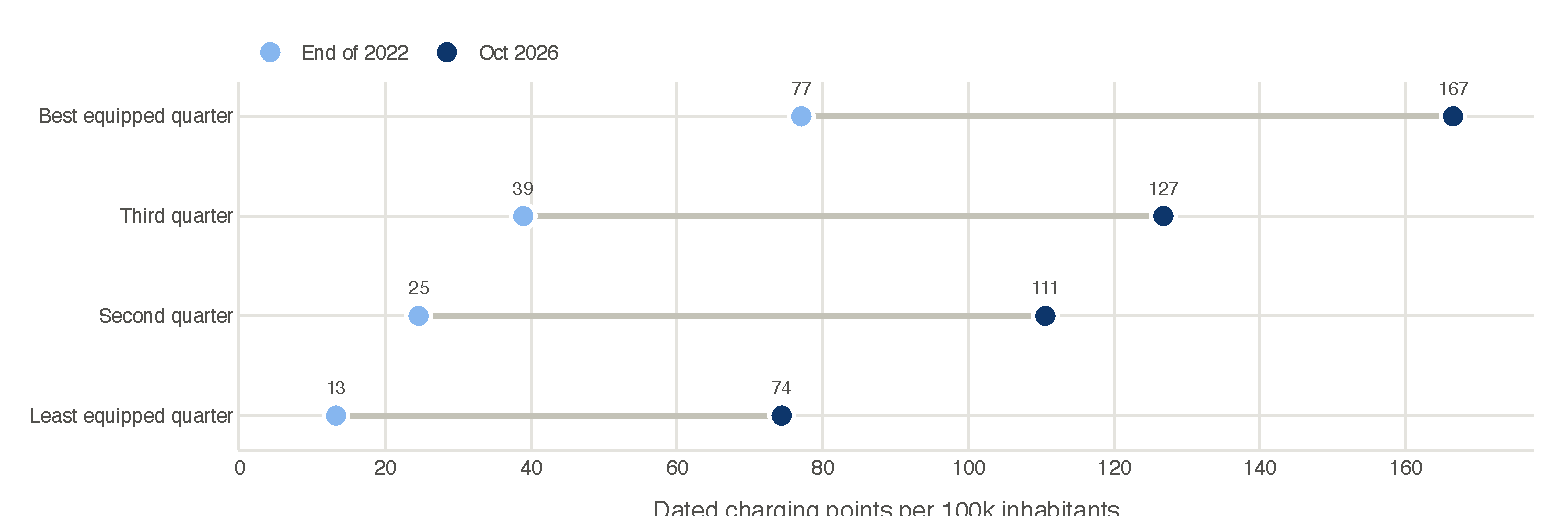
\includegraphics[width=0.92\linewidth]{figures/convergence.pdf}
\caption{Dated points per 100,000 inhabitants at the end of \nPivotYear{} (light) and in \nEndMonth{} (dark), by quarter of départements.}
\end{figure}

The least equipped quarter went from \nConvLowBefore{} to \nConvLowAfter{} dated points per 100,000 people, while the best equipped quarter went from \nConvHighBefore{} to \nConvHighAfter. The overseas départements did not follow: together they added \nOverAdded{} dated points since \nStartYear, \nOverPace{} per 100,000 inhabitants a year against \nMainPace{} on the mainland. On the mainland, the slowest catch-up is in \nSlowestName: at \nSlowestPace{} dated points per 100,000 a year it would need \nSlowestYears{} years to reach today's national level. Undated points are not counted in the pace, so this is an upper bound.

\section{App design}

\textbf{Narrative.} The page follows the arc of the brief: a hook (the national figure next to \nLowestName), context (KPIs and timeline), insights (map, rural versus dense, EV ownership, catch-up) and implications. Each section opens with a one-sentence headline built from the data, so the text changes with the filters. The introduction and conclusions always use national figures, so the story stays stable while the user explores.

\textbf{Controls.} The sidebar has area and départements, commissioning period, whether to count undated points, power class, operators, and the indicator shown on the map and ranking. The period has one meaning everywhere: snapshot views show the network at the end of the period, and growth counts points added inside it. Undated points can only be counted when the period ends in the current year, since they cannot be placed in the past. Empty selections show a message instead of an empty chart.

\textbf{Performance and reproducibility.} The raw files (about 170 MB) are never loaded by the app. \texttt{data/fetch\_data.py} downloads them with a cache and writes about 1 MB of parquet and GeoJSON, which the app loads through \texttt{st.cache\_data}. Thresholds, seeds, palette and policy dates live in \texttt{config.py}; dependencies are pinned. The app was tested from a clean virtual environment and on several hundred random filter combinations without error.

\textbf{Accessibility.} Power classes use a single-hue ordinal blue ramp and maps a single-hue sequential scale, both checked for colour-vision deficiency and contrast. Every chart has a text description and, where useful, a data table, so no value depends on colour alone. Every axis has a label and a unit.

\section{Limitations}

\begin{itemize}
  \item Publication is declarative. Operators publish their own files, some late or not at all, so a low figure can mean missing data rather than missing chargers. This matters most overseas.
  \item \nDateMissingPct\% of points have no commissioning date. Time charts and the convergence analysis use the \nDatedPct\% that do. Removed points leave no trace, so closures are invisible.
  \item Battery-electric and plug-in hybrid cars are counted together, at the holder's address.
  \item Département averages hide what happens inside a département.
  \item All relations between EV ownership and charging are correlations. The app makes no causal claim.
  \item data.gouv.fr announces that this consolidated file will be replaced by the national base on transport.data.gouv.fr and removed after 31 December 2026.
\end{itemize}

\section{Implications and next steps}

On the mainland the question has moved from ``is there a charger'' to ``is there the right charger in the right place''. A département-level average will rarely flag a shortage there; planners will learn more at commune or EPCI scale, from fast charging in dense areas where many drivers cannot charge at home, and from usage data. Overseas, the first step is to check whether local operators declare their points on data.gouv.fr.

Next steps for the analysis: join the dynamic IRVE feed to measure use rather than presence, split the vehicle register into battery-electric and plug-in hybrid cars to apply the two AFIR ratios, add the national road network to test the motorway question, and repeat the analysis at EPCI level.

\section*{References}
\small
\begin{itemize}[leftmargin=*]
  \item IRVE consolidated file: \url{https://www.data.gouv.fr/fr/datasets/fichier-consolide-des-bornes-de-recharge-pour-vehicules-electriques/}
  \item Schema: \url{https://schema.data.gouv.fr/etalab/schema-irve-statique/}
  \item Vehicle register by commune (Agence ORE): \url{https://www.data.gouv.fr/datasets/voitures-particulieres-immatriculees-par-commune-et-par-type-de-recharge-jeu-de-donnees-aaadata}
  \item Insee reference populations: \url{https://www.data.gouv.fr/datasets/populations-de-reference}
  \item Administrative contours: \url{https://www.data.gouv.fr/datasets/contours-administratifs}
  \item LOM law, loi n° 2019-1428: \url{https://www.legifrance.gouv.fr/jorf/id/JORFTEXT000039666574}
  \item Arrêté du 4 mai 2021: \url{https://www.legifrance.gouv.fr/jorf/id/JORFTEXT000043475441}
  \item Avere-France, 100,000 public points: \url{https://www.avere-france.org/wp-content/uploads/2023/05/CP-100-000-points-de-recharge.pdf}
  \item Regulation (EU) 2023/1804 (AFIR): \url{https://eur-lex.europa.eu/eli/reg/2023/1804/oj}
\end{itemize}

\end{document}
